\documentclass[twoside]{book}

% Packages required by doxygen
\usepackage{fixltx2e}
\usepackage{calc}
\usepackage{doxygen}
\usepackage[export]{adjustbox} % also loads graphicx
\usepackage{graphicx}
\usepackage[utf8]{inputenc}
\usepackage{makeidx}
\usepackage{multicol}
\usepackage{multirow}
\PassOptionsToPackage{warn}{textcomp}
\usepackage{textcomp}
\usepackage[nointegrals]{wasysym}
\usepackage[table]{xcolor}

% Font selection
\usepackage[T1]{fontenc}
\usepackage[scaled=.90]{helvet}
\usepackage{courier}
\usepackage{amssymb}
\usepackage{sectsty}
\renewcommand{\familydefault}{\sfdefault}
\allsectionsfont{%
  \fontseries{bc}\selectfont%
  \color{darkgray}%
}
\renewcommand{\DoxyLabelFont}{%
  \fontseries{bc}\selectfont%
  \color{darkgray}%
}
\newcommand{\+}{\discretionary{\mbox{\scriptsize$\hookleftarrow$}}{}{}}

% Page & text layout
\usepackage{geometry}
\geometry{%
  a4paper,%
  top=2.5cm,%
  bottom=2.5cm,%
  left=2.5cm,%
  right=2.5cm%
}
\tolerance=750
\hfuzz=15pt
\hbadness=750
\setlength{\emergencystretch}{15pt}
\setlength{\parindent}{0cm}
\setlength{\parskip}{3ex plus 2ex minus 2ex}
\makeatletter
\renewcommand{\paragraph}{%
  \@startsection{paragraph}{4}{0ex}{-1.0ex}{1.0ex}{%
    \normalfont\normalsize\bfseries\SS@parafont%
  }%
}
\renewcommand{\subparagraph}{%
  \@startsection{subparagraph}{5}{0ex}{-1.0ex}{1.0ex}{%
    \normalfont\normalsize\bfseries\SS@subparafont%
  }%
}
\makeatother

% Headers & footers
\usepackage{fancyhdr}
\pagestyle{fancyplain}
\fancyhead[LE]{\fancyplain{}{\bfseries\thepage}}
\fancyhead[CE]{\fancyplain{}{}}
\fancyhead[RE]{\fancyplain{}{\bfseries\leftmark}}
\fancyhead[LO]{\fancyplain{}{\bfseries\rightmark}}
\fancyhead[CO]{\fancyplain{}{}}
\fancyhead[RO]{\fancyplain{}{\bfseries\thepage}}
\fancyfoot[LE]{\fancyplain{}{}}
\fancyfoot[CE]{\fancyplain{}{}}
\fancyfoot[RE]{\fancyplain{}{\bfseries\scriptsize Generated by Doxygen }}
\fancyfoot[LO]{\fancyplain{}{\bfseries\scriptsize Generated by Doxygen }}
\fancyfoot[CO]{\fancyplain{}{}}
\fancyfoot[RO]{\fancyplain{}{}}
\renewcommand{\footrulewidth}{0.4pt}
\renewcommand{\chaptermark}[1]{%
  \markboth{#1}{}%
}
\renewcommand{\sectionmark}[1]{%
  \markright{\thesection\ #1}%
}

% Indices & bibliography
\usepackage{natbib}
\usepackage[titles]{tocloft}
\setcounter{tocdepth}{3}
\setcounter{secnumdepth}{5}
\makeindex

% Hyperlinks (required, but should be loaded last)
\usepackage{ifpdf}
\ifpdf
  \usepackage[pdftex,pagebackref=true]{hyperref}
\else
  \usepackage[ps2pdf,pagebackref=true]{hyperref}
\fi
\hypersetup{%
  colorlinks=true,%
  linkcolor=blue,%
  citecolor=blue,%
  unicode%
}

% Custom commands
\newcommand{\clearemptydoublepage}{%
  \newpage{\pagestyle{empty}\cleardoublepage}%
}

\usepackage{caption}
\captionsetup{labelsep=space,justification=centering,font={bf},singlelinecheck=off,skip=4pt,position=top}

%===== C O N T E N T S =====

\begin{document}

% Titlepage & ToC
\hypersetup{pageanchor=false,
             bookmarksnumbered=true,
             pdfencoding=unicode
            }
\pagenumbering{alph}
\begin{titlepage}
\vspace*{7cm}
\begin{center}%
{\Large libcollect }\\
\vspace*{1cm}
{\large Generated by Doxygen 1.8.13}\\
\end{center}
\end{titlepage}
\clearemptydoublepage
\pagenumbering{roman}
\tableofcontents
\clearemptydoublepage
\pagenumbering{arabic}
\hypersetup{pageanchor=true}

%--- Begin generated contents ---
\chapter{libcollect}
\label{index}\hypertarget{index}{}{\ttfamily libcollect} is a C library of useful collection types. So far I have only implemented a hash map. Because this is C these types are pretty unsafe and use {\ttfamily void $\ast$}s everywhere. The pointers these containers store should be allocated on the heap as they will be freed when the containers are freed.

\subsection*{Types}


\begin{DoxyItemize}
\item \hyperlink{structmap}{map}
\end{DoxyItemize}

\subsection*{License}

This project is released in the public domain. 
\chapter{Deprecated List}
\label{deprecated}
\Hypertarget{deprecated}

\begin{DoxyRefList}
\item[\label{deprecated__deprecated000001}%
\Hypertarget{deprecated__deprecated000001}%
Member \hyperlink{map_8h_a62aecb5aad4e2d9da77fff653e1ad57b}{M\+A\+P\+\_\+\+U\+S\+E\+D\+\_\+\+AT} (m, i)]Used map\+\_\+exists instead 
\end{DoxyRefList}
\chapter{Class Index}
\section{Class List}
Here are the classes, structs, unions and interfaces with brief descriptions\+:\begin{DoxyCompactList}
\item\contentsline{section}{\hyperlink{structmap}{map} \\*A simple hashmap }{\pageref{structmap}}{}
\item\contentsline{section}{\hyperlink{structmap__node}{map\+\_\+node} }{\pageref{structmap__node}}{}
\end{DoxyCompactList}

\chapter{File Index}
\section{File List}
Here is a list of all files with brief descriptions\+:\begin{DoxyCompactList}
\item\contentsline{section}{include/collect/\hyperlink{hash_8h}{hash.\+h} }{\pageref{hash_8h}}{}
\item\contentsline{section}{include/collect/\hyperlink{map_8h}{map.\+h} }{\pageref{map_8h}}{}
\end{DoxyCompactList}

\chapter{Class Documentation}
\hypertarget{structmap}{}\section{map Struct Reference}
\label{structmap}\index{map@{map}}


A simple hashmap.  




{\ttfamily \#include $<$map.\+h$>$}



Collaboration diagram for map\+:\nopagebreak
\begin{figure}[H]
\begin{center}
\leavevmode
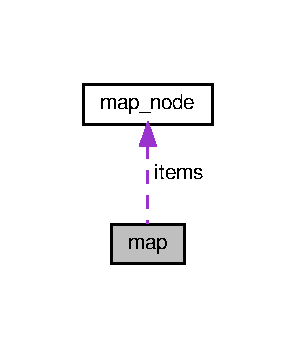
\includegraphics[width=142pt]{structmap__coll__graph}
\end{center}
\end{figure}
\subsection*{Public Attributes}
\begin{DoxyCompactItemize}
\item 
uint64\+\_\+t \hyperlink{structmap_a5598721b26d57cba0a9d1fb346b62101}{len}
\item 
\hyperlink{structmap__node}{map\+\_\+node} $\ast$ \hyperlink{structmap_a6b38d0a3f8cdff696c5907a53e9f2e42}{items}
\item 
uint64\+\_\+t \hyperlink{structmap_ac907ec19ab9a47454f8192671935f22b}{full}
\item 
uint64\+\_\+t \hyperlink{structmap_a5b34954e76b42c69e8dcc257579ef504}{count}
\end{DoxyCompactItemize}


\subsection{Detailed Description}
A simple hashmap. 

Allocate map with \hyperlink{map_8h_a5193bc7b8432d7e2873579aa63185c27}{new\+\_\+map()} and free it with \hyperlink{map_8h_a55b5ea441f2e33b216dbb120d188626b}{free\+\_\+map()}. Items can be added with \hyperlink{map_8h_aa0a79fdac7a6bbbdab1ecd26c9903e45}{map\+\_\+set()} or the \hyperlink{map_8h_aab70789517583a1c42a66f69dcd14dba}{M\+A\+P\+\_\+\+S\+E\+T()} macro. \hyperlink{map_8h_a8254246acf42bdc32d6e53e17708bcf3}{map\+\_\+exists()} can be used to check if an item exists in the map, \hyperlink{map_8h_aa6bbe7b3686e1bd7f87b86ab48dad6db}{map\+\_\+get()} and \hyperlink{map_8h_a79b7329d2be1fe2b7298e56e53365116}{M\+A\+P\+\_\+\+G\+E\+T()} can be used to retrieve items. 

\subsection{Member Data Documentation}
\mbox{\Hypertarget{structmap_a5b34954e76b42c69e8dcc257579ef504}\label{structmap_a5b34954e76b42c69e8dcc257579ef504}} 
\index{map@{map}!count@{count}}
\index{count@{count}!map@{map}}
\subsubsection{\texorpdfstring{count}{count}}
{\footnotesize\ttfamily uint64\+\_\+t map\+::count}

\mbox{\Hypertarget{structmap_ac907ec19ab9a47454f8192671935f22b}\label{structmap_ac907ec19ab9a47454f8192671935f22b}} 
\index{map@{map}!full@{full}}
\index{full@{full}!map@{map}}
\subsubsection{\texorpdfstring{full}{full}}
{\footnotesize\ttfamily uint64\+\_\+t map\+::full}

\mbox{\Hypertarget{structmap_a6b38d0a3f8cdff696c5907a53e9f2e42}\label{structmap_a6b38d0a3f8cdff696c5907a53e9f2e42}} 
\index{map@{map}!items@{items}}
\index{items@{items}!map@{map}}
\subsubsection{\texorpdfstring{items}{items}}
{\footnotesize\ttfamily \hyperlink{structmap__node}{map\+\_\+node}$\ast$ map\+::items}

\mbox{\Hypertarget{structmap_a5598721b26d57cba0a9d1fb346b62101}\label{structmap_a5598721b26d57cba0a9d1fb346b62101}} 
\index{map@{map}!len@{len}}
\index{len@{len}!map@{map}}
\subsubsection{\texorpdfstring{len}{len}}
{\footnotesize\ttfamily uint64\+\_\+t map\+::len}



The documentation for this struct was generated from the following file\+:\begin{DoxyCompactItemize}
\item 
include/collect/\hyperlink{map_8h}{map.\+h}\end{DoxyCompactItemize}

\hypertarget{structmap__node}{}\section{map\+\_\+node Struct Reference}
\label{structmap__node}\index{map\+\_\+node@{map\+\_\+node}}


{\ttfamily \#include $<$map.\+h$>$}

\subsection*{Public Attributes}
\begin{DoxyCompactItemize}
\item 
char $\ast$ \hyperlink{structmap__node_a7f78daf7b510166b7d2c0d15c0f155d8}{key}
\item 
void $\ast$ \hyperlink{structmap__node_a1d4251143de664ac95bbeb48d0323f1b}{val}
\item 
int \hyperlink{structmap__node_a879076d62a4f4f9deb75feffc6fd1940}{used}\+: 1
\item 
uint32\+\_\+t \hyperlink{structmap__node_a1cf8a340a58c73cb61b837208417a09d}{h}
\end{DoxyCompactItemize}


\subsection{Member Data Documentation}
\mbox{\Hypertarget{structmap__node_a1cf8a340a58c73cb61b837208417a09d}\label{structmap__node_a1cf8a340a58c73cb61b837208417a09d}} 
\index{map\+\_\+node@{map\+\_\+node}!h@{h}}
\index{h@{h}!map\+\_\+node@{map\+\_\+node}}
\subsubsection{\texorpdfstring{h}{h}}
{\footnotesize\ttfamily uint32\+\_\+t map\+\_\+node\+::h}

\mbox{\Hypertarget{structmap__node_a7f78daf7b510166b7d2c0d15c0f155d8}\label{structmap__node_a7f78daf7b510166b7d2c0d15c0f155d8}} 
\index{map\+\_\+node@{map\+\_\+node}!key@{key}}
\index{key@{key}!map\+\_\+node@{map\+\_\+node}}
\subsubsection{\texorpdfstring{key}{key}}
{\footnotesize\ttfamily char$\ast$ map\+\_\+node\+::key}

\mbox{\Hypertarget{structmap__node_a879076d62a4f4f9deb75feffc6fd1940}\label{structmap__node_a879076d62a4f4f9deb75feffc6fd1940}} 
\index{map\+\_\+node@{map\+\_\+node}!used@{used}}
\index{used@{used}!map\+\_\+node@{map\+\_\+node}}
\subsubsection{\texorpdfstring{used}{used}}
{\footnotesize\ttfamily int map\+\_\+node\+::used}

\mbox{\Hypertarget{structmap__node_a1d4251143de664ac95bbeb48d0323f1b}\label{structmap__node_a1d4251143de664ac95bbeb48d0323f1b}} 
\index{map\+\_\+node@{map\+\_\+node}!val@{val}}
\index{val@{val}!map\+\_\+node@{map\+\_\+node}}
\subsubsection{\texorpdfstring{val}{val}}
{\footnotesize\ttfamily void$\ast$ map\+\_\+node\+::val}



The documentation for this struct was generated from the following file\+:\begin{DoxyCompactItemize}
\item 
include/collect/\hyperlink{map_8h}{map.\+h}\end{DoxyCompactItemize}

\chapter{File Documentation}
\hypertarget{hash_8h}{}\section{include/collect/hash.h File Reference}
\label{hash_8h}\index{include/collect/hash.\+h@{include/collect/hash.\+h}}
{\ttfamily \#include $<$stdint.\+h$>$}\newline
Include dependency graph for hash.\+h\+:\nopagebreak
\begin{figure}[H]
\begin{center}
\leavevmode
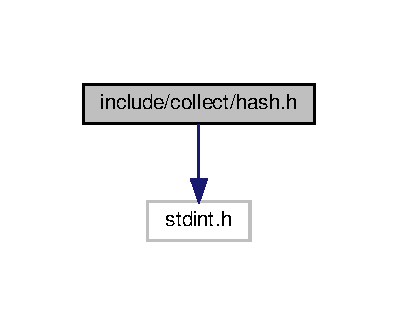
\includegraphics[width=191pt]{hash_8h__incl}
\end{center}
\end{figure}
This graph shows which files directly or indirectly include this file\+:\nopagebreak
\begin{figure}[H]
\begin{center}
\leavevmode
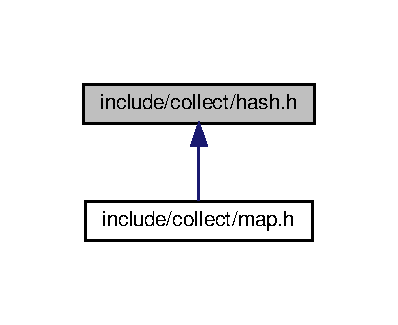
\includegraphics[width=191pt]{hash_8h__dep__incl}
\end{center}
\end{figure}
\subsection*{Functions}
\begin{DoxyCompactItemize}
\item 
uint32\+\_\+t \hyperlink{hash_8h_a684f16ef7d061a29ac01a28bf70398d5}{hash} (char $\ast$str)
\end{DoxyCompactItemize}


\subsection{Function Documentation}
\mbox{\Hypertarget{hash_8h_a684f16ef7d061a29ac01a28bf70398d5}\label{hash_8h_a684f16ef7d061a29ac01a28bf70398d5}} 
\index{hash.\+h@{hash.\+h}!hash@{hash}}
\index{hash@{hash}!hash.\+h@{hash.\+h}}
\subsubsection{\texorpdfstring{hash()}{hash()}}
{\footnotesize\ttfamily uint32\+\_\+t hash (\begin{DoxyParamCaption}\item[{char $\ast$}]{str }\end{DoxyParamCaption})}


\hypertarget{map_8h}{}\section{include/collect/map.h File Reference}
\label{map_8h}\index{include/collect/map.\+h@{include/collect/map.\+h}}
{\ttfamily \#include $<$stdint.\+h$>$}\newline
{\ttfamily \#include $<$stdlib.\+h$>$}\newline
{\ttfamily \#include \char`\"{}collect/hash.\+h\char`\"{}}\newline
Include dependency graph for map.\+h\+:\nopagebreak
\begin{figure}[H]
\begin{center}
\leavevmode
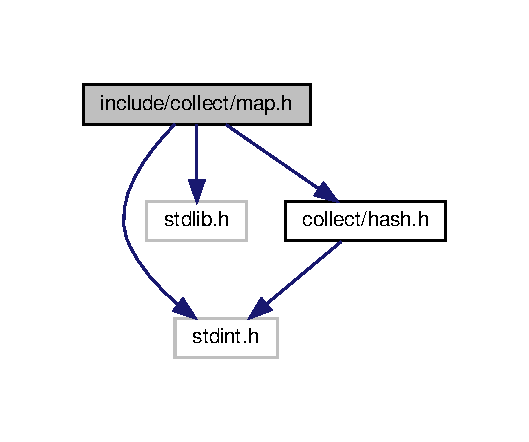
\includegraphics[width=254pt]{map_8h__incl}
\end{center}
\end{figure}
\subsection*{Classes}
\begin{DoxyCompactItemize}
\item 
struct \hyperlink{structmap__node}{map\+\_\+node}
\item 
struct \hyperlink{structmap}{map}
\begin{DoxyCompactList}\small\item\em A simple hashmap. \end{DoxyCompactList}\end{DoxyCompactItemize}
\subsection*{Macros}
\begin{DoxyCompactItemize}
\item 
\#define \hyperlink{map_8h_ac50b211fd9943433fce0412401ee53b3}{M\+A\+P\+\_\+\+A\+L\+L\+O\+C\+\_\+\+S\+I\+ZE}~(1 $\ast$ 1024)
\item 
\#define \hyperlink{map_8h_aefa63a937c01506d31bfee242f788aa7}{E\+M\+P\+T\+Y\+\_\+\+N\+O\+DE}~\{ N\+U\+LL, N\+U\+LL, 0, 0 \}
\item 
\#define \hyperlink{map_8h_a62aecb5aad4e2d9da77fff653e1ad57b}{M\+A\+P\+\_\+\+U\+S\+E\+D\+\_\+\+AT}(m,  i)~(m\mbox{[}i\mbox{]}.used)
\item 
\#define \hyperlink{map_8h_a79b7329d2be1fe2b7298e56e53365116}{M\+A\+P\+\_\+\+G\+ET}(t,  m,  k)~$\ast$(t $\ast$)\hyperlink{map_8h_aa6bbe7b3686e1bd7f87b86ab48dad6db}{map\+\_\+get}(m, k)
\item 
\#define \hyperlink{map_8h_aab70789517583a1c42a66f69dcd14dba}{M\+A\+P\+\_\+\+S\+ET}(m,  k,  v)
\begin{DoxyCompactList}\small\item\em Helper macro to allocate memory for a value on the heap and store it at a given key. \end{DoxyCompactList}\end{DoxyCompactItemize}
\subsection*{Typedefs}
\begin{DoxyCompactItemize}
\item 
typedef struct \hyperlink{structmap__node}{map\+\_\+node} \hyperlink{map_8h_ad33aac071d8efb2032b564970286165e}{map\+\_\+node}
\item 
typedef struct \hyperlink{structmap}{map} \hyperlink{map_8h_a598bfbfd73f0b9e15e943e3f76785218}{map}
\end{DoxyCompactItemize}
\subsection*{Functions}
\begin{DoxyCompactItemize}
\item 
\hyperlink{structmap}{map} $\ast$ \hyperlink{map_8h_a5193bc7b8432d7e2873579aa63185c27}{new\+\_\+map} ()
\begin{DoxyCompactList}\small\item\em Allocate a new map on the heap. \end{DoxyCompactList}\item 
\hyperlink{structmap}{map} $\ast$ \hyperlink{map_8h_ae8a2458fea6554c519b508cdd053582b}{new\+\_\+map\+\_\+sized} (uint64\+\_\+t)
\begin{DoxyCompactList}\small\item\em Allocate a map on the heap with a specific capacity. Map will be reallocated if this capacity is exceeded. \end{DoxyCompactList}\item 
void \hyperlink{map_8h_a55b5ea441f2e33b216dbb120d188626b}{free\+\_\+map} (\hyperlink{structmap}{map} $\ast$m)
\begin{DoxyCompactList}\small\item\em Free a map on the heap. \end{DoxyCompactList}\item 
void \hyperlink{map_8h_aa0a79fdac7a6bbbdab1ecd26c9903e45}{map\+\_\+set} (\hyperlink{structmap}{map} $\ast$m, char $\ast$k, void $\ast$v)
\begin{DoxyCompactList}\small\item\em Set a certain value in the map. \end{DoxyCompactList}\item 
void $\ast$ \hyperlink{map_8h_aa6bbe7b3686e1bd7f87b86ab48dad6db}{map\+\_\+get} (\hyperlink{structmap}{map} $\ast$m, char $\ast$k)
\begin{DoxyCompactList}\small\item\em Get the value in a map by it\textquotesingle{}s key. \end{DoxyCompactList}\item 
int \hyperlink{map_8h_a8254246acf42bdc32d6e53e17708bcf3}{map\+\_\+exists} (\hyperlink{structmap}{map} $\ast$m, char $\ast$k)
\begin{DoxyCompactList}\small\item\em Check if a key is used in a map. \end{DoxyCompactList}\item 
void \hyperlink{map_8h_a3a87bba4af6dfe8179516f26ba56c5f9}{map\+\_\+debug} (\hyperlink{structmap}{map} $\ast$m)
\begin{DoxyCompactList}\small\item\em Print a map\textquotesingle{}s contents to stdout. \end{DoxyCompactList}\end{DoxyCompactItemize}


\subsection{Macro Definition Documentation}
\mbox{\Hypertarget{map_8h_aefa63a937c01506d31bfee242f788aa7}\label{map_8h_aefa63a937c01506d31bfee242f788aa7}} 
\index{map.\+h@{map.\+h}!E\+M\+P\+T\+Y\+\_\+\+N\+O\+DE@{E\+M\+P\+T\+Y\+\_\+\+N\+O\+DE}}
\index{E\+M\+P\+T\+Y\+\_\+\+N\+O\+DE@{E\+M\+P\+T\+Y\+\_\+\+N\+O\+DE}!map.\+h@{map.\+h}}
\subsubsection{\texorpdfstring{E\+M\+P\+T\+Y\+\_\+\+N\+O\+DE}{EMPTY\_NODE}}
{\footnotesize\ttfamily \#define E\+M\+P\+T\+Y\+\_\+\+N\+O\+DE~\{ N\+U\+LL, N\+U\+LL, 0, 0 \}}

\mbox{\Hypertarget{map_8h_ac50b211fd9943433fce0412401ee53b3}\label{map_8h_ac50b211fd9943433fce0412401ee53b3}} 
\index{map.\+h@{map.\+h}!M\+A\+P\+\_\+\+A\+L\+L\+O\+C\+\_\+\+S\+I\+ZE@{M\+A\+P\+\_\+\+A\+L\+L\+O\+C\+\_\+\+S\+I\+ZE}}
\index{M\+A\+P\+\_\+\+A\+L\+L\+O\+C\+\_\+\+S\+I\+ZE@{M\+A\+P\+\_\+\+A\+L\+L\+O\+C\+\_\+\+S\+I\+ZE}!map.\+h@{map.\+h}}
\subsubsection{\texorpdfstring{M\+A\+P\+\_\+\+A\+L\+L\+O\+C\+\_\+\+S\+I\+ZE}{MAP\_ALLOC\_SIZE}}
{\footnotesize\ttfamily \#define M\+A\+P\+\_\+\+A\+L\+L\+O\+C\+\_\+\+S\+I\+ZE~(1 $\ast$ 1024)}

\mbox{\Hypertarget{map_8h_a79b7329d2be1fe2b7298e56e53365116}\label{map_8h_a79b7329d2be1fe2b7298e56e53365116}} 
\index{map.\+h@{map.\+h}!M\+A\+P\+\_\+\+G\+ET@{M\+A\+P\+\_\+\+G\+ET}}
\index{M\+A\+P\+\_\+\+G\+ET@{M\+A\+P\+\_\+\+G\+ET}!map.\+h@{map.\+h}}
\subsubsection{\texorpdfstring{M\+A\+P\+\_\+\+G\+ET}{MAP\_GET}}
{\footnotesize\ttfamily \#define M\+A\+P\+\_\+\+G\+ET(\begin{DoxyParamCaption}\item[{}]{t,  }\item[{}]{m,  }\item[{}]{k }\end{DoxyParamCaption})~$\ast$(t $\ast$)\hyperlink{map_8h_aa6bbe7b3686e1bd7f87b86ab48dad6db}{map\+\_\+get}(m, k)}

\mbox{\Hypertarget{map_8h_aab70789517583a1c42a66f69dcd14dba}\label{map_8h_aab70789517583a1c42a66f69dcd14dba}} 
\index{map.\+h@{map.\+h}!M\+A\+P\+\_\+\+S\+ET@{M\+A\+P\+\_\+\+S\+ET}}
\index{M\+A\+P\+\_\+\+S\+ET@{M\+A\+P\+\_\+\+S\+ET}!map.\+h@{map.\+h}}
\subsubsection{\texorpdfstring{M\+A\+P\+\_\+\+S\+ET}{MAP\_SET}}
{\footnotesize\ttfamily \#define M\+A\+P\+\_\+\+S\+ET(\begin{DoxyParamCaption}\item[{}]{m,  }\item[{}]{k,  }\item[{}]{v }\end{DoxyParamCaption})}

{\bfseries Value\+:}
\begin{DoxyCode}
\{                                                            \(\backslash\)
        \_\_typeof\_\_(v) *\_\_map\_temp = malloc(\textcolor{keyword}{sizeof}(\_\_typeof(v))); \(\backslash\)
        *\_\_map\_temp = v;                                         \(\backslash\)
        map\_set(m, k, \_\_map\_temp);                               \(\backslash\)
    \}
\end{DoxyCode}


Helper macro to allocate memory for a value on the heap and store it at a given key. 

\begin{DoxyWarning}{Warning}
This is unsafe and should be used with caution, especially for more complex types 
\end{DoxyWarning}

\begin{DoxyParams}{Parameters}
{\em m} & The map \\
\hline
{\em k} & The key at which to insert the value \\
\hline
{\em v} & The value \\
\hline
\end{DoxyParams}
\mbox{\Hypertarget{map_8h_a62aecb5aad4e2d9da77fff653e1ad57b}\label{map_8h_a62aecb5aad4e2d9da77fff653e1ad57b}} 
\index{map.\+h@{map.\+h}!M\+A\+P\+\_\+\+U\+S\+E\+D\+\_\+\+AT@{M\+A\+P\+\_\+\+U\+S\+E\+D\+\_\+\+AT}}
\index{M\+A\+P\+\_\+\+U\+S\+E\+D\+\_\+\+AT@{M\+A\+P\+\_\+\+U\+S\+E\+D\+\_\+\+AT}!map.\+h@{map.\+h}}
\subsubsection{\texorpdfstring{M\+A\+P\+\_\+\+U\+S\+E\+D\+\_\+\+AT}{MAP\_USED\_AT}}
{\footnotesize\ttfamily \#define M\+A\+P\+\_\+\+U\+S\+E\+D\+\_\+\+AT(\begin{DoxyParamCaption}\item[{}]{m,  }\item[{}]{i }\end{DoxyParamCaption})~(m\mbox{[}i\mbox{]}.used)}

\begin{DoxyRefDesc}{Deprecated}
\item[\hyperlink{deprecated__deprecated000001}{Deprecated}]Used map\+\_\+exists instead \end{DoxyRefDesc}


\subsection{Typedef Documentation}
\mbox{\Hypertarget{map_8h_a598bfbfd73f0b9e15e943e3f76785218}\label{map_8h_a598bfbfd73f0b9e15e943e3f76785218}} 
\index{map.\+h@{map.\+h}!map@{map}}
\index{map@{map}!map.\+h@{map.\+h}}
\subsubsection{\texorpdfstring{map}{map}}
{\footnotesize\ttfamily typedef struct \hyperlink{structmap}{map} \hyperlink{structmap}{map}}

\mbox{\Hypertarget{map_8h_ad33aac071d8efb2032b564970286165e}\label{map_8h_ad33aac071d8efb2032b564970286165e}} 
\index{map.\+h@{map.\+h}!map\+\_\+node@{map\+\_\+node}}
\index{map\+\_\+node@{map\+\_\+node}!map.\+h@{map.\+h}}
\subsubsection{\texorpdfstring{map\+\_\+node}{map\_node}}
{\footnotesize\ttfamily typedef struct \hyperlink{structmap__node}{map\+\_\+node} \hyperlink{structmap__node}{map\+\_\+node}}



\subsection{Function Documentation}
\mbox{\Hypertarget{map_8h_a55b5ea441f2e33b216dbb120d188626b}\label{map_8h_a55b5ea441f2e33b216dbb120d188626b}} 
\index{map.\+h@{map.\+h}!free\+\_\+map@{free\+\_\+map}}
\index{free\+\_\+map@{free\+\_\+map}!map.\+h@{map.\+h}}
\subsubsection{\texorpdfstring{free\+\_\+map()}{free\_map()}}
{\footnotesize\ttfamily void free\+\_\+map (\begin{DoxyParamCaption}\item[{\hyperlink{structmap}{map} $\ast$}]{m }\end{DoxyParamCaption})}



Free a map on the heap. 


\begin{DoxyParams}{Parameters}
{\em m} & The map to free \\
\hline
\end{DoxyParams}
\mbox{\Hypertarget{map_8h_a3a87bba4af6dfe8179516f26ba56c5f9}\label{map_8h_a3a87bba4af6dfe8179516f26ba56c5f9}} 
\index{map.\+h@{map.\+h}!map\+\_\+debug@{map\+\_\+debug}}
\index{map\+\_\+debug@{map\+\_\+debug}!map.\+h@{map.\+h}}
\subsubsection{\texorpdfstring{map\+\_\+debug()}{map\_debug()}}
{\footnotesize\ttfamily void map\+\_\+debug (\begin{DoxyParamCaption}\item[{\hyperlink{structmap}{map} $\ast$}]{m }\end{DoxyParamCaption})}



Print a map\textquotesingle{}s contents to stdout. 

\begin{DoxyWarning}{Warning}
Should not be used in production 
\end{DoxyWarning}

\begin{DoxyParams}{Parameters}
{\em m} & The map \\
\hline
\end{DoxyParams}
\mbox{\Hypertarget{map_8h_a8254246acf42bdc32d6e53e17708bcf3}\label{map_8h_a8254246acf42bdc32d6e53e17708bcf3}} 
\index{map.\+h@{map.\+h}!map\+\_\+exists@{map\+\_\+exists}}
\index{map\+\_\+exists@{map\+\_\+exists}!map.\+h@{map.\+h}}
\subsubsection{\texorpdfstring{map\+\_\+exists()}{map\_exists()}}
{\footnotesize\ttfamily int map\+\_\+exists (\begin{DoxyParamCaption}\item[{\hyperlink{structmap}{map} $\ast$}]{m,  }\item[{char $\ast$}]{k }\end{DoxyParamCaption})}



Check if a key is used in a map. 


\begin{DoxyParams}{Parameters}
{\em m} & The map \\
\hline
{\em k} & The key \\
\hline
\end{DoxyParams}
\begin{DoxyReturn}{Returns}
1 if the key is used, 0 otherwise 
\end{DoxyReturn}
\mbox{\Hypertarget{map_8h_aa6bbe7b3686e1bd7f87b86ab48dad6db}\label{map_8h_aa6bbe7b3686e1bd7f87b86ab48dad6db}} 
\index{map.\+h@{map.\+h}!map\+\_\+get@{map\+\_\+get}}
\index{map\+\_\+get@{map\+\_\+get}!map.\+h@{map.\+h}}
\subsubsection{\texorpdfstring{map\+\_\+get()}{map\_get()}}
{\footnotesize\ttfamily void$\ast$ map\+\_\+get (\begin{DoxyParamCaption}\item[{\hyperlink{structmap}{map} $\ast$}]{m,  }\item[{char $\ast$}]{k }\end{DoxyParamCaption})}



Get the value in a map by it\textquotesingle{}s key. 


\begin{DoxyParams}{Parameters}
{\em m} & The map \\
\hline
{\em k} & The key \\
\hline
\end{DoxyParams}
\begin{DoxyReturn}{Returns}
The value at k 
\end{DoxyReturn}
\mbox{\Hypertarget{map_8h_aa0a79fdac7a6bbbdab1ecd26c9903e45}\label{map_8h_aa0a79fdac7a6bbbdab1ecd26c9903e45}} 
\index{map.\+h@{map.\+h}!map\+\_\+set@{map\+\_\+set}}
\index{map\+\_\+set@{map\+\_\+set}!map.\+h@{map.\+h}}
\subsubsection{\texorpdfstring{map\+\_\+set()}{map\_set()}}
{\footnotesize\ttfamily void map\+\_\+set (\begin{DoxyParamCaption}\item[{\hyperlink{structmap}{map} $\ast$}]{m,  }\item[{char $\ast$}]{k,  }\item[{void $\ast$}]{v }\end{DoxyParamCaption})}



Set a certain value in the map. 


\begin{DoxyParams}{Parameters}
{\em m} & The map \\
\hline
{\em k} & The key whose value should be changed \\
\hline
{\em v} & The new value \\
\hline
\end{DoxyParams}
\mbox{\Hypertarget{map_8h_a5193bc7b8432d7e2873579aa63185c27}\label{map_8h_a5193bc7b8432d7e2873579aa63185c27}} 
\index{map.\+h@{map.\+h}!new\+\_\+map@{new\+\_\+map}}
\index{new\+\_\+map@{new\+\_\+map}!map.\+h@{map.\+h}}
\subsubsection{\texorpdfstring{new\+\_\+map()}{new\_map()}}
{\footnotesize\ttfamily \hyperlink{structmap}{map}$\ast$ new\+\_\+map (\begin{DoxyParamCaption}{ }\end{DoxyParamCaption})}



Allocate a new map on the heap. 

\begin{DoxyReturn}{Returns}
A pointer to the allocated map 
\end{DoxyReturn}
\mbox{\Hypertarget{map_8h_ae8a2458fea6554c519b508cdd053582b}\label{map_8h_ae8a2458fea6554c519b508cdd053582b}} 
\index{map.\+h@{map.\+h}!new\+\_\+map\+\_\+sized@{new\+\_\+map\+\_\+sized}}
\index{new\+\_\+map\+\_\+sized@{new\+\_\+map\+\_\+sized}!map.\+h@{map.\+h}}
\subsubsection{\texorpdfstring{new\+\_\+map\+\_\+sized()}{new\_map\_sized()}}
{\footnotesize\ttfamily \hyperlink{structmap}{map}$\ast$ new\+\_\+map\+\_\+sized (\begin{DoxyParamCaption}\item[{uint64\+\_\+t}]{ }\end{DoxyParamCaption})}



Allocate a map on the heap with a specific capacity. Map will be reallocated if this capacity is exceeded. 

\begin{DoxyReturn}{Returns}
A pointer to the allocated map 
\end{DoxyReturn}

\hypertarget{README_8md}{}\section{R\+E\+A\+D\+M\+E.\+md File Reference}
\label{README_8md}\index{R\+E\+A\+D\+M\+E.\+md@{R\+E\+A\+D\+M\+E.\+md}}

%--- End generated contents ---

% Index
\backmatter
\newpage
\phantomsection
\clearemptydoublepage
\addcontentsline{toc}{chapter}{Index}
\printindex

\end{document}
